\documentclass[]{article}

%opening
\title{TMR: Detecting Structure in Graphical Data}
\author{Lawrence Tray \\ Ioannis Kontoyiannis}

%packages
\usepackage[margin=0.5in]{geometry}
\usepackage{graphicx}
\usepackage{amsmath}
\usepackage{amssymb}
\usepackage{hyperref}
\usepackage{caption}
\usepackage{subcaption}
\usepackage{mathtools}
\usepackage{parskip}
\usepackage{fancyvrb}
\usepackage{bbm}
\usepackage{algorithm}% http://ctan.org/pkg/algorithm
\usepackage{algpseudocode}% http://ctan.org/pkg/algorithmicx

%bibliography
\usepackage[backend=bibtex]{biblatex}
\addbibresource{interim-sources.bib}

%package setup
\graphicspath{{./img/}}
\DeclareMathOperator*{\argmax}{arg\,max}
\DeclareMathOperator*{\argmin}{arg\,min}

%custom commands
\newcommand{\dft}{\mathcal{F}}
\newcommand{\idft}{\mathcal{F}^{-1}}
\newcommand{\Xcal}{\mathcal{X}}
\newcommand{\Dcal}{\mathcal{D}}
\newcommand{\cmplx}{\mathbb{C}}
\newcommand{\E}{\mathbb{E}}
\newcommand{\Gaussian}{\mathcal{N}}
\newcommand{\Gcal}{\mathcal{G}}
\newcommand{\Vcal}{\mathcal{V}}
\newcommand{\Ecal}{\mathcal{E}}
\newcommand{\pbold}{\boldsymbol{p}}
\newcommand{\sigmabold}{\boldsymbol{\sigma}}
\newcommand{\lik}{\mathcal{L}}
\newcommand{\kl}{\mathcal{D}}
\newcommand{\Integers}{\mathbb{Z}}
\newcommand{\SBM}{\textrm{SBM}}
\newcommand{\iid}{\stackrel{iid}{\sim}}
\newcommand{\one}{\mathbbm{1}}
\newcommand{\figwidth}{0.4\linewidth}


% definition
\newtheorem{definition}{Definition}[section]
\newtheorem{theorem}{Theorem}[section]
\newtheorem{corollary}{Corollary}[theorem]
\newtheorem{lemma}[theorem]{Lemma}


\begin{document}

\maketitle

\begin{abstract}
This is the Technical Milestone Report for the II-B project: detecting structure in graphical data. We produce vast quantities of graphical data every day and yet the techniques used to analyse their structure are still in their infancy. We start by defining the Stochastic Block Model (SBM) widely used in academia and develop a theorem to verify structure in a given labelled graph.
\end{abstract}

\tableofcontents

\section{Introduction}

There is a wealth of graphical data in the world and more is being produced each second; social networks, website hyperlinks and academic collaborations are just some examples of this data. There is a wealth of algorithms developed to analyse graphical data. Nevertheless, that same principled framework we have for querying classical data (hypothesis testing) is less developed for graphical data. Do my friends vote the same way I do or do researchers collaborate with those of the same gender? We want to answer these questions and not only that, we wish to report our confidence in the answers. To that end there is space to expand the hypothesis testing framework to graphs.

\section{The Stochastic Block Model}

The most popular graphical model in industry and indeed academia is called the Stochastic Block Model (SBM). We use a definition adapted from Abbe \cite{Abbe}.

\begin{definition}
	\label{defn:sbm}
	Let $n \in \Integers^+$ be the number of vertices and $k \in \Integers^+$ be the number of communities in an SBM graph. We define a probability vector $\pi = [\pi_1, \pi_2 \dots \pi_k]^T$ to be the prior on the k-communities. Each vertex $v \in \Vcal = \{1, 2 \dots N\}$ has a community label $X_v \in \{1, 2 \dots n\}$. Let $W$ be a symmetric $k \times k$ matrix with entries in $[0,1]$ called the connectivity matrix. We say that the pair $(X, \Gcal) \sim \textrm{SBM}(n, \pi, W)$ if X is an $N$-dimensional vector with each component independently distributed as the community prior $X_v \sim \pi$ and $\Gcal$ is an $N$-vertex graph where each pair of vertices $(i, j)$ is connected with probability $p(i \leftrightarrow j) = W_{X_i, X_j}$ independently of other pairs of vertices. Lastly, we define the community sets as $\Omega_i = \Omega_i(X) \coloneqq \{v \in \Vcal : X_v = i\}$ which contains all vertices belonging to community $i$.
\end{definition}

Though the definition of the SBM is simple, it allows for very deep and rich analysis of graphical datasets. For certain problems it helps to define the symmetric SBM.

\begin{definition}
	\label{defn:sym-sbm}
	The symmetric SBM is a special case denoted by $\textrm{SSBM}(n, k, q_{in}, q_{out}) \equiv \textrm{SBM}(n, p, W)$ if the community prior $p$ is uniform ($p_i = 1/k$ for $i \in \{1, 2, \dots k\}$) and $W_{ij}$ takes only two values, one on diagonal and another off diagonal such that $W_{ij} = q_{in}$ for $i=j$ and $W_{ij} = q_{out}$ for $i \neq j$.
\end{definition}

\section{Verifying Structure}
\subsection{Theory}

Armed with this definition we tackle the simplest problem in structure verification. Given an undirected graph $\Gcal$ and vertex-labels $X$, we wish to determine whether the two communities $a$ and $b$ connect differently. Put formally, this is a hypothesis test on the parameters of $W$. There are three parameters we would wish to test: $W_{aa}, W_{ab}$ and $W_{bb}$ (note that for an undirected graph $W = W^T$ necessarily so $W_{ab} = W_{ba}$). To do this we can perform three-pairwise hypothesis tests. Here we test $W_{\alpha}$ against $W_{\beta}$ where $\alpha$ and $\beta$ are unique indices in $\{(a,a), (a, b), (b,b)\}$:
%
\begin{equation}
\begin{aligned}
	H_0:& \quad W_{\alpha} = W_{\beta} \\
	H_1:& \quad W_{\alpha} \neq W_{\beta}
\end{aligned}
\end{equation}

We formulate this as a likelihood ratio test. Letting $\lik(\Dcal | H)$ denote the likelihood of observing the data $\Dcal = (X, G)$ under hypothesis $H$. Therefore, the test statistic is given by:
%
\begin{equation}
	t_n \coloneqq \log \frac{\lik(\Dcal | H_1)}{\lik(\Dcal | H_0)}
	\label{eqn:test-statistic-start}
\end{equation}

At this point it helps to introduce some more notation. We define the number of vertices in community $i$ by $n_i \coloneqq |\Omega_i(X)|$ leading to the result $n = \sum_i n_i$. Furthermore, we use $E_{ij} = E_{ij}(X, \Gcal)$ to denote the number of realised edges between communities $i$ and $j$ (in generality $i$ may be equal to $j$) and similarly define $M_{ij} = M_{ij}(X)$ as the maximum number of possible edges between the communities. For an undirected graph this can be computed simply as follows:
%
\begin{equation}
	M_{ij} = M_{ij} (X) = \begin{cases}
		n_i n_j &\text{for } i \neq j \\
		\frac{1}{2}n_i (n_i - 1) &\text{for } i = j
	\end{cases}
\end{equation}

With this new notation, the likelihood function can be written explicitly:
%
\begin{align}
\lik(\Dcal | H) &= p(X| \pi) \cdot p(\Gcal | W, X) \nonumber \\
&= p(X | \pi) \cdot \prod_{i=1}^{k} \prod_{j=i}^{k} p(E_{ij} | W, X) \nonumber \\
&= p(X | \pi) \cdot \prod_{i=1}^{k} \prod_{j=i}^{k} W_{ij} ^ {E_{ij}} \cdot \left( 1 - W_{ij} \right) ^ {(M_{ij} - E_{ij})}
\label{eqn:likelihood-verbose}
\end{align}

The form of $p(\Gcal | W, X)$ is simply a sequence of Bernoulli trials for each distinct community pair $(i, j)$ (edge present with probability $W_{ij}$ or edge absent with probability $1 - W_{ij}$ for every pair of vertices across those communities). A sequence of Bernoullis is the same as a Binomial distribution without the combinatoric term. By inspecting equation \ref{eqn:likelihood-verbose} we see that only terms involving $W_{\alpha}$ and $W_{\beta}$ are going to differ under the two hypotheses; the rest of the terms will cancel in our calculation of the test-statistic $t_n$. Therefore, we can rewrite the likelihood as follows:
%
\begin{equation}
	\lik (\Dcal | H) \propto f (W_\alpha, E_\alpha, M_\alpha) \cdot f (W_\beta, E_\beta, M_\beta)
\end{equation} 
\begin{equation}
	\textrm{where } f (w, e, m) \coloneqq w^e \cdot (1-w)^{(m - e)}
	\label{eqn:f-defn}
\end{equation}

We note that $f(w, e, m)$ is simply the probability of observing a specific sequence of $e$ successes in $m$ independent Bernoulli trials with parameter $w$. Its maximiser with respect to the first argument is easily computed through partial differentiation giving:
%
\begin{equation}
	\argmax_w f(w, e, m) = \hat{w} = e / m
	\label{eqn:f-maximiser}
\end{equation}

Furthermore, we spot the following property $f(w, e_1, m_1) \cdot f(w, e_2, m_2) = f(w, e_1 + e_2, m_1 + m_2)$ or in other words, the function $f$ is linear in its second and third arguments given the same first argument. As such we can manipulate equation \ref{eqn:test-statistic-start} greatly to give:
%
\begin{align}
	t_n &= \log \frac
	{
		\max_{W_{\alpha} \neq W_{\beta}}(f (W_\alpha, E_\alpha, M_\alpha) \cdot f (W_\beta, E_\beta, M_\beta))
	}
	{
		\max_{W_\alpha = W_\beta} (f (W_\alpha, E_\alpha, M_\alpha) \cdot f (W_\beta, E_\beta, M_\beta))
	} \nonumber \\
	&= \log \frac{
		\max_p f(p, E_\alpha, M_\alpha) \cdot \max_q f(q, E_\alpha, M_\alpha)
	}{
		\max_r f(r, E_\alpha + E_\beta, M_\alpha + M_\beta)
	} \nonumber \\
	&= \log \frac{f(\hat{p}, E_\alpha, M_\alpha)}{f(\hat{r}, E_\alpha, M_\alpha)} + \log \frac{f(\hat{q}, E_\beta, M_\beta)}{f(\hat{r}, E_\beta, M_\beta)}
\end{align}

Where $\hat{p} \coloneqq E_\alpha / M_\alpha$, $\hat{q} \coloneqq E_\beta / M_\beta$ and $\hat{r} \coloneqq (E_\alpha + E_\beta) / (M_\alpha + M_\beta)$. These symbols are introduced to make the notation more succinct.

\begin{lemma}[KL divergence]
	With $f$ defined as in equation \ref{eqn:f-defn}, $0 \leq e \leq m$ and $r \in [0, 1]$ it holds that:
	%
	\begin{equation*}
		\log \frac{f(e/m, e, m)}{f(r, e, m)} = m \cdot \kl \left( \textrm{Bern}(e/m) || \textrm{Bern}(r) \right)
	\end{equation*}

	where $\kl(g || h)$ is the Kullback-Leibler divergence between two probability mass functions $g, h: \Xcal \mapsto [0, 1]$. $\kl$ is defined in discrete space as $\kl(g || h) \coloneqq \sum_{x \in \Xcal} g(x) \log \frac{g(x)}{h(x)}$ and $\textrm{Bern(p)}$ denotes the Bernoulli p.m.f with parameter $p$.
	\label{lem:kl-div}
\end{lemma}

Proving lemma \ref{lem:kl-div} is simply a case of algebraic manipulation:
%
\begin{align}
	\log \frac{f(e/m, e, m)}{f(r, e, m)} &= e \cdot \log \frac{e/m}{r} + (m-e) \cdot \log \frac{1- e/m}{1 - r} \nonumber \\
	&= m \cdot \left( (e/m) \cdot \log \frac{e/m}{r} + (1 - e/m) \cdot \log \frac{1- e/m}{1 - r} \right) \nonumber \\
	&= m \kl \left( \textrm{Bern}(e/m) || \textrm{Bern}(r) \right) \quad \therefore \textrm{QED}
\end{align}

Thereby proving lemma \ref{lem:kl-div}. This allows us to simplify the test-statistic into a form that is more numerically stable:
%
\begin{equation}
	t_n = M_\alpha \cdot \kl\left( \textrm{Bern}(\hat{p}) || \textrm{Bern}(\hat{r})\right) + 
	M_\beta \cdot \kl\left( \textrm{Bern}(\hat{q}) || \textrm{Bern}(\hat{r})\right)
	\label{eqn:test-stat-compute-form}
\end{equation}

However, we must simplify further still.
%
\begin{lemma}[$\chi^2$ approximation]
	\label{lem:kl-approx-chi}
	For $g(x) \approx h(x)$ then $\kl(g || h) \approx \frac{1}{2} \chi^2(g || h)$ where $\chi^2$ is the chi-squared distance between two distributions defined as $\chi^2(g || h) \coloneqq \sum_{x \in \Xcal} \frac{(g(x)-h(x))^2}{h(x)}$ 
\end{lemma}

The proof requires defining $\delta(x) \coloneqq g(x) - h(x)$ and taking a Taylor expansion of $\log 1 + x$:
%
\begin{align*}
	\kl(g||h) &= \sum_{x \in \Xcal} (\delta + h) \log \left(1 + \frac{\delta}{g} \right) 
	= \sum_{x \in \Xcal} (\delta + h) \left( \frac{\delta}{h} - \frac{\delta^2}{2h^2} + O(\delta^3) \right)  \\
	&= \sum_{x \in \Xcal} \delta + \frac{1}{2} \sum_{x \in \Xcal} \frac{\delta^2}{h} + O(\delta^3) 
	= \frac{1}{2} \sum_{x \in \Xcal} \frac{\delta^2}{h} + O(\delta^3) \\
	&= \frac{1}{2} \chi^2(g||h) + O(\delta^3) \approx \frac{1}{2} \chi^2(h||g) \quad \therefore \textrm{QED}
\end{align*}
%
Where the summation over $\delta$ evaluates to 0 because $\delta$ is the difference of two valid p.m.f's which each sum to 1 over $x \in \Xcal$. We are able to neglect the $O(\delta^3)$ terms for $g$ very close to $h$. The chi-squared distance between two Bernoullis for $g = Bern(p)$ and $h = Bern(q)$ is simply:
%
\begin{equation}
\chi^2(\textrm{Bern}(p) || \textrm{Bern}(q)) = \left( \frac{p-q}{\sqrt{q(1-q)}} \right)^2
\end{equation}

We can apply these results to equation \ref{eqn:test-stat-compute-form} to obtain an approximate expression for $t_n$ under the null for large $n$ such that $\hat{p}$, $\hat{q}$ and $\hat{r}$ are all close meaning Lemma \ref{lem:kl-approx-chi} is valid, giving:
%
\begin{align}
	t_n &\approx \frac{1}{2 \hat{r}(1 - \hat{r})} \left( 
	M_\alpha \left(\hat{p} - \hat{r}\right)^2 +
	M_\beta \left(\hat{q} - \hat{r} \right)^2 
	\right) \nonumber \\
	&= \frac{1}{2 \hat{r}(1-\hat{r})} \left( 
	M_\alpha \left(\frac{M_\alpha (\hat{p} - \hat{q})}{M_\alpha + M_\beta} \right)^2 +
	M_\beta \left(\frac{M_\beta (\hat{q} - \hat{p})}{M_\alpha + M_\beta} \right)^2
	\right) \nonumber \\
	&= \frac{1}{2} \left( \frac{\hat{p} - \hat{q}}{\sqrt{\hat{r}(1- \hat{r})(1/M_\alpha + 1/M_\beta)}} \right)^2
	= \frac{1}{2} z_n^2
\end{align}

Through application of the Central Limit Theorem (CLT) and Slutsky's Theorem it can be shown that as $n \rightarrow \infty$ under the null $H_0$ the term in brackets on the final line is distributed like a standard Gaussian $z_n \sim \Gaussian(0,1)$. This is because under the same assumptions, assuming that $W_\alpha = W_\beta = \mu$, by the CLT $\hat{p} \sim (\mu, \mu(1 - \mu)/ M_\alpha)$, $\hat{q} \sim (\mu, \mu(1 - \mu)/ M_\beta)$ and $\hat{p} \sim (\mu, \mu(1 - \mu)/ (M_\alpha + M_\beta))$. Therefore, the whole test-statistic is distributed as $t_n \sim \frac{1}{2} \chi^2_1$ by the definition of the $\chi^2_p$ distribution: $\chi^2_p \sim \sum_{i=1}{p} Z_i^2$ for $Z_i \sim \Gaussian(0,1)$. This leads to the following theorem:

\begin{theorem}[$\chi^2$ test]
	For $(X, \Gcal) \sim \textrm{SBM}(n, p, W)$, given the realised graph and class labels $(X, \Gcal)$ we can perform a hypothesis test on parameters $W_\alpha$ and $W_\beta$ of the connectivity matrix $W$.
	%
	\begin{align*}
	H_0:& \quad W_{\alpha} = W_{\beta} \\
	H_1:& \quad W_{\alpha} \neq W_{\beta}
	\end{align*}
	If the log-likelihood ratio test statistic $t_n$ is computed as in equation \ref{eqn:test-stat-compute-form}, repeated here:
	%
	\begin{equation*}
		t_n \coloneqq  M_\alpha \cdot \kl\left( \textrm{Bern}(\hat{p}) || \textrm{Bern}(\hat{r})\right) + 
		M_\beta \cdot \kl\left( \textrm{Bern}(\hat{q}) || \textrm{Bern}(\hat{r})\right)
	\end{equation*}
	
	Where $\hat{p} \coloneqq E_\alpha / M_\alpha$, $\hat{q} \coloneqq E_\beta / M_\beta$ and $\hat{r} \coloneqq (E_\alpha + E_\beta) / (M_\alpha + M_\beta)$. Then as the number of vertices $n \rightarrow \infty, t_n \sim \frac{1}{2} \chi^2_1$ under the null $H_0$. Therefore, we reject $H_0$ at the $100(\zeta)\%$ confidence level if and only if $2t_n \geq \psi^{-1}(\zeta)$, where $\psi^{-1}$ is the $\chi^2_1$ inverse cdf satisfying $Pr(Y \leq \psi^{-1}(\zeta)) = \zeta$ given $Y \sim \chi^2_1$.
	
	\label{theorem:hyp-test-sbm-chi}
\end{theorem}

\begin{corollary}[z-test]
	We can also use a slightly simpler test-statistic $z_n$ albeit with some loss of generality. If we define $z_n$ to be:
	%
	\begin{equation*}
		z_n \coloneqq \frac{\hat{p} - \hat{q}}{\sqrt{\hat{r}(1- \hat{r})(1/M_\alpha + 1/M_\beta)}}
	\end{equation*}
	
	With the symbols retaining their previous meanings. Under the null $H_0$, as $n \rightarrow \infty$ then $z_n \sim \Gaussian(0, 1)$. Meaning that, we can construct a similar test to reject $H_0$ at the $100(\zeta)\%$ confidence level if and only if $|z_n| \geq \phi^{-1}(\zeta)$, where $\phi^{-1}$ is the standard inverse Gaussian cdf on magnitude satisfying $Pr(|Y| \leq \phi^{-1}(\zeta)) = \zeta$ given $Y \sim \Gaussian(0, 1)$
\end{corollary}

\subsection{Early results}

We seek to apply theorem \ref{theorem:hyp-test-sbm-chi} to various real-world graphical datasets. We start by analysing social network graphs. The Stanford Network Analysis Project (SNAP for short) \cite{snapnets} offers a wealth of Facebook egonets. An egonet is simply a graph where all vertices (in this case each representing a Facebook user) are guaranteed to be connected to one central node (the ego-node). The data consists of the undirected set of edges $\Gcal$ indicating whether any two vertices (Facebook users) are connected (friends on Facebook). We also have a set of binary labels for each vertex $X$. However, for the sake of privacy these features are anonymised. This is best explained through the example below: \\

\begin{center}
\begin{minipage}{8cm}
\begin{Verbatim}[fontsize=\small, frame=single, label={\fbox{Example anonymised feature flags}}]
75 first_name;anonymized feature 75
76 first_name;anonymized feature 76
77 gender;anonymized feature 77
78 gender;anonymized feature 78
79 hometown;id;anonymized feature 79
\end{Verbatim}
\end{minipage}
\end{center}


Each feature is anonymised to avoid disclosing personally identifiable information. I cannot tell whether vertex $v$ is male or female but I can tell whether they are the same gender as another vertex $w$ which suffices for our analysis. If we have a total of $f$ features and $n$ vertices, then the feature matrix $X$ would be an $n \times f$ where each row is the feature vector for the corresponding vertex. The features are binary such that $X_{ij} \in \{0, 1\}$ indicating the feature of and on respectively.

We perform a hypothesis test in the manner described by theorem \ref{theorem:hyp-test-sbm-chi} to determine whether gender influences how friends connect on Facebook. We choose to analyse SNAP egonet with id 0 (the id of the egonet is the id of the single egonode) though any choice is possible. The egonet is plotted on figure \ref{fig:ego-0-by-gender}. We use the Python package NetworkX \cite{networkx} for its visualisation tools. Indeed, we will discuss layout algorithms later as for now we focus on the simple hypothesis test.
%
\begin{figure}[!h]
	\centering
	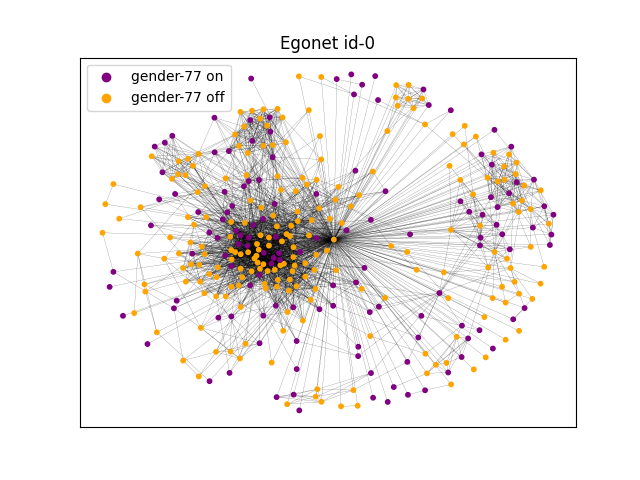
\includegraphics[width=\figwidth]{ego-0-by-gender.png}
	\caption{Egonet 0 with nodes coloured by gender}
	\label{fig:ego-0-by-gender}
\end{figure}

We use an SBM model with $k=2$ communities (1: gender-77 on and 2: gender-77 off) to model the egonet and perform a three-way hypothesis test on the parameters of the connectivity Matrix $W$.
%
\begin{equation}
	W = \begin{bmatrix}
		p_1 & q \\
		q & p_2
	\end{bmatrix}
\end{equation}

Therefore, $p_1$ is the probability that two vertices of gender-77 are connected, $q$ is the crossover probability and $p_2$ is the connection probability within the gender-78 community. The results of the hypothesis tests are given in table \ref{tab:egonet-0-hyp-tests} alongside p-values (we choose a 95\% significance level to reject the null). However, in some cases the test statistics were so extreme that the p-value saturated to 0.
%
\begin{table}[!h]
	\centering
	\begin{tabular}{c c c c c}
		$n_1$                & $n_2$                & $\hat{p_1}$ & $\hat{q}$ & $\hat{p_2}$       \\ \hline
		130 & 218 & $8.13 \times 10^{-2}$ & $7.66 \times 10^{-2}$ & $10.6 \times 10^{-2}$
	\end{tabular}
	\caption{Egonet-0 properties and parameter estimates}
	\label{tab:egonet-0-props}
\end{table}

\begin{table}[!h]
	\centering
	\begin{tabular}{cccccc}
		Test & $H_0$                & $H_1$                & p-value & $H_0$ rejected       \\ \hline
		1    & $p_1 = q$            & $p_1 \neq q$         & 0.158 &  No                \\
		2    & $p_1 = p_2$ & $p_1 \neq p_2$ & 0.000 & Yes \\
		3    & $q = p_2$ & $q \neq p_2$ &  0.000 & Yes
	\end{tabular}
	\caption{Egonet-0 hypothesis tests that gender influences friendship formation}
	\label{tab:egonet-0-hyp-tests}
\end{table}

Test 2 being rejected gives evidence that one gender has on average more friends from their own gender. We see that gender-78 people (community 2) have on average more friends ($\hat{p_2} > \hat{p_1}$ in table \ref{tab:egonet-0-props}). The rejection of the null in test 3 gives evidence that gender-78 treat gender-77 people differently to their own gender. Indeed, a gender-78 person is more likely to be friends with a fellow 78-er than with a 77-er. However, we do not reject the null in test 1 so there is insufficient evidence to claim the reverse (that 77-ers tend to stay away from 78-ers). Nevertheless, these are results on a single egonet so can hardly be generalised to society as a whole. However, the exercise has highlighted some interesting points:

\begin{enumerate}
	\item The hypothesis test framework does not quantify the magnitude of the difference just whether or not a difference exists.
	\item As the degree $n$ increases, the p-values will necessarily become more extreme.
	\item The method relies on the analyst to specify the features of interest so results may be misleading if third variables are missing from the analysis.
\end{enumerate} 

To address these shortcomings we instead approach the problem from a different angle. For now we have been given a graph with fully labelled vertices and ask if a given feature affect the structure. Instead, we could take a graph and partition into communities first (without using feature information) and then ask which features most reliably explain the partition. For that we need a way of detecting structure.

\section{Detecting Structure}
\subsection{Weak recovery}

This is the problem of recovering the communities from the graph $\Gcal$. We use the notation $\hat{X}$ to denote the produced estimate of the community labels for the $n$ vertices. Obviously, if the SBM is symmetric then we must allow for an arbitrary relabelling of the communities $r: \{1, 2 \dots k\} \mapsto \{1, 2 \dots k\}$ before we compare the agreement of the two vectors $\hat{X}$ and $X$. The agreement $A$ and normalised agreement $\tilde{A}$ between two vectors $x, y$ are computed as below:
%
\begin{align}
	A(x, y) &= \max_r \frac{1}{n} \sum_{i=1}^{n} \one (x_i, r(y_i)) \\
	\tilde{A}(x, y) &= \max_r \frac{1}{k} \sum_{i=1}^{k} \frac{1}{n_i} \sum_{v \in \Omega_i(x)} \one(x_v, r(y_v))
\end{align}

The normalised agreement is important for asymmetric SBMs as it takes the agreement averaged over communities rather than vertices. We define 4 recovery regimes (plus the trivial no recovery), such that the following holds (adapted from Abbe \cite{Abbe}):

\begin{definition}[Recovery regimes]
	for $(X, \Gcal) \sim \textrm{SBM}(m, p, W)$ the following recovery requirements are solved if there exists an algorithm which takes $\Gcal$ and input and outputs a vector of classifications $\hat{X} = \hat{X}(\Gcal)$ such that as $n \rightarrow \infty$:
	\begin{itemize}
		\item \textbf{Exact recovery:} $Pr\{A(X, \hat{X}) = 1\} = 1 - o(1)$ correct classification recovered almost surely
		\item \textbf{Almost exact recovery:} $Pr\{A(X, \hat{X}) = 1 - o(1)\} = 1 - o(1)$ vanishing fraction misclassified almost surely
		\item \textbf{Partial recovery:} $Pr\{\tilde{A}(X, \hat{X}) \geq \alpha\} = 1 - o(1), 1 > \alpha > 1/k$ better than choosing from uniform prior
		\item \textbf{Weak recovery:} $Pr\{\tilde{A}(X, \hat{X}) \geq 1/k + \epsilon \} = 1 - o(1), \epsilon > 0$ marginally better than choosing from uniform prior
		\item \textbf{No recovery:} graph provides no information as to class labels
	\end{itemize}
	Where $o(1)$ denotes a family of functions that tend to 0 as $n \rightarrow \infty$. The regime $\Gcal$ occupies depends on the parameters of the SBM. Each recovery regime is weaker than the one above it so Exact recovery implies weak recovery is possible..
\end{definition}

We choose to focus on weak recovery as it is the least strict of all regimes. An alternative statement of weak recovery is given below:

\begin{definition}[Weak recovery]
	\label{defn:weak-recovery}
	for  $(X, \Gcal) \sim \textrm{SBM}(n, p, W)$ weak recovery is solved if there exists $\epsilon > 0$ and a certain choice of indices $i, j \in \{1, 2 \dots k\}$ and an algorithm that takes as input $\Gcal$ and outputs a partition of the vertex set $\Vcal$ into two distinct sets $S$ and $S^C$ (detected communities 1 and 2 respectively) such that:
	\begin{equation*}
		Pr\left\{ \frac{|\Omega_i \cap S|}{|\Omega_i|} - \frac{|\Omega_j \cap S|}{|\Omega_j|} \geq \epsilon \right\} = 1 - o(1)
	\end{equation*}

	Bearing in mind the definition of $\Omega_i = \Omega_i(X) \coloneqq \{v \in \Vcal : X_v = i\}$. In other words, we require the partition $S \subset \Vcal$ to cut across communities such that the fraction of a particular community in partition $S$ with respect to the whole community is different for a choice of two communities.  
\end{definition}


One of the most promising weak recovery algorithms is called Acyclic Belief Propagataion (ABP). This is a message-passing algorithm that solves weak recovery in the sense of definition \ref{defn:weak-recovery}. Algorithm \ref{alg:lin-abp} is heavily adapated from Abbe and Sandon \cite{Linear-ABP}. The original paper goes into much more detail but it works on the premise that one can infer the community of a particular vertex by taking a majority vote among the  of all its neighbours. The algorithm is non-determinsitic and requires the vertex set $\Vcal = \Vcal(\Gcal)$ and edge set $\Ecal = \Ecal(\Gcal)$ as well as two hyper-parameters $r$ (the maximum cyclic length to correct for) and $T$ (the number of iterations):

%
\begin{algorithm}
	\caption{Linearised Acyclic Belief Propagation (ABP)}
	\label{alg:lin-abp}
	\begin{algorithmic}
		\Function{ABP}{$\Ecal$, $\Vcal$, r, T}
		\State $y^{(0)}_{v' \rightarrow v} \gets \Gaussian(0, 1)$ \Comment{Initialise messages randomly}
		\For{$t \in \{1, 2 \cdots T\}$}
		\For{$(v, v') \in \Ecal$}
		\State $s^{(t-1)} \gets \frac{1}{2|E|} \sum_{(v, v') \in \Ecal} y^{(t-1)}_{v' \rightarrow v}$ \Comment{Compute average}
		\State $z^{(t-1)}_{v' \rightarrow v} \gets y^{(t-1)}_{v' \rightarrow v} - s^{(t-1)}$ \Comment{Recentre messages}
		\State $y^{(t)}_{v' \rightarrow v} \gets \sum_{(v', v'') \in \Ecal \setminus \{v\}}z^{(t-1)}_{v'' \rightarrow v'}$ \Comment{Sum incoming messages} \\
		\If {$\exists v''' \in \Vcal$ such that $(v''' \rightarrow v \rightarrow v')$ is on a cycle of length $r' \leq r$}
		\State $y^{(t)}_{v' \rightarrow v} \leftarrow y^{(t)}_{v' \rightarrow v} - \sum_{(v, v'') \in \Ecal \setminus \{v', v'''\}}z^{(t-r')}_{v'' \rightarrow v'}$ \Comment{Cyclic correction}
		\EndIf
		\EndFor
		\EndFor
		\State $\sigma_v = \sum_{(v, v') \in \Ecal} y^{(T)}_{v' \rightarrow v}$ \Comment{Sum incoming messages}
		\State $\hat{X}_v \gets 1$ if $\sigma_v > 0$ else $2$ \Comment{Hard assignment}
		\State \textbf{return} $\hat{X}_v$
		\EndFunction
	\end{algorithmic}
\end{algorithm}

We implement this algorithm in Python and apply it to the Facebook Egonets described earlier. We found that the hyperparameter settings $r=3$ and $T=5$ yielded good results. We define the normalised ABP output below:
%
\begin{equation}
	\tilde{\sigma}_v \coloneqq \begin{cases}
		\frac{\sigma_v}{|\sigma_{max}|} \textrm{ for } \sigma_j > 0 \\
		\frac{\sigma_v}{|\sigma_{min}|} \textrm{ for } \sigma_j \leq 0
	\end{cases}
\end{equation}

Where $\sigma_{max}$ is the largest positive value of $\sigma_v$ and $\sigma_{min}$ is the most negative. The normalised quantity $\tilde{\sigma}_v \in [-1, +1]$ with $0$ still being the midpoint that determines which detected community vertex $v$ is assigned to. We colour each vertex according to this quantity $\tilde{\sigma}_v$ and plot the graph on figure \ref{fig:abp-output-norm}. We see intuitively that ABP has worked. The blue cluster in the lower right is clearly part of one community and a great many vertices do not seem to belong to any cluster at all so their classification is uncertain (the colour is close to green).
%
\begin{figure}[!h]
	\centering
	\begin{subfigure}{0.4\linewidth}
		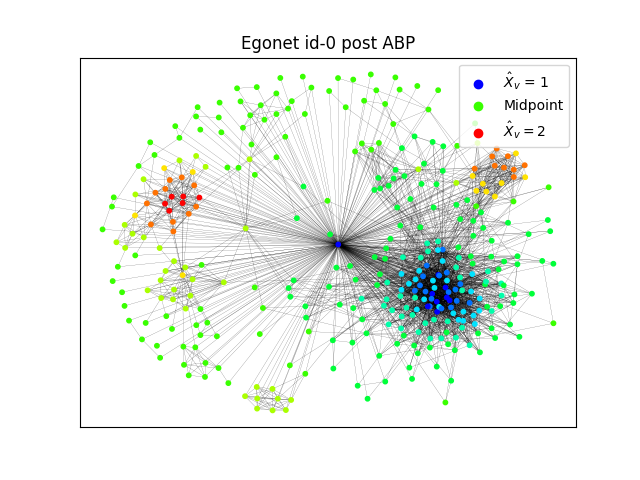
\includegraphics[width=\linewidth]{ego-0-abp.png}
		\caption{Normalised ABP output $\tilde{\sigma}_v$ colouring vertices}
		\label{fig:abp-output-norm}
	\end{subfigure}
	\begin{subfigure}{0.4\linewidth}
		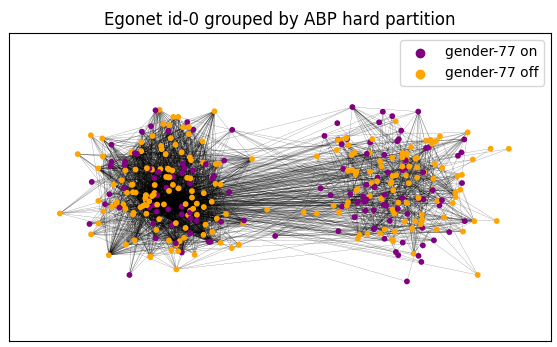
\includegraphics[width=\linewidth]{ego-0-abp-by-gender.png}
		\caption{Vertices grouped by hard ABP assignments and coloured by gender. In assigned community 1 ($S$ - left) we have \{58, 122\} gender-77 and gender-78 respectively and in detected community 2 ($S^C$ - right) we have \{72, 96\}}
		\label{fig:abp-output-by-gender}
	\end{subfigure}
	\caption{Egonet-0 weak recovery results}
\end{figure}

We can evaluate formally whether weak recovery has succeeded by inspecting figure \ref{fig:abp-output-by-gender} and treating gender-77 and gender-78 as the two communities of interest:
%
\begin{equation}
	\frac{|\Omega_{77} \cap S|}{|\Omega_{77}|} = \frac{58}{58+72} = 0.446
	\quad \textrm{and} \quad
	 \frac{|\Omega_{78} \cap S|}{|\Omega_{78}|} = \frac{122}{122+96} = 0.560
\end{equation}

Clearly the fraction of each community in the partition $S$ differ substantially so we say that weak recovery is solved. The set $S$ contains a higher proportion of the overall 78-population than of the 77-population.

\subsection{From detection to inference}

We now have an algorithm (ABP) that partitions our graph into two sets that are most readily explained by an SBM with $k=2$ communities. We can now ask the question of which vertex labels most readily explain the separation. Therefore, we can determine which features have the largest impact on the graphical structure; this circumvents the binary resolution problem with the hypothesis testing approach.

This part of the project is still in its early stages so these are just preliminary results. For reference we plot the community fractions in the detected set $S$
\footnote{ABP is non-deterministic so each subplot is the result of a different run of ABP. Subfigures use the same partition $S$ but no exact comparison is possible between figures.}
on figure \ref{fig:abp-output-community-fractions}. It is interesting to note that if two bars on this plot differ substantially then we have satisfied the requirment for weak recovery as defined in \ref{defn:weak-recovery}. We necessarily remove the constraint on the community sets $\Omega_i$ to be disjoint as one vertex can have multiple features turned on. This can be modelled more precisely through a Mixed Membership Model but for now an SBM with $k=2$ communities suffices.

We perform a linear regression on the normalised ABP output $\tilde{\sigma}_v$
%
\begin{figure}[!h]
	\centering
	\begin{subfigure}{0.6\linewidth}
		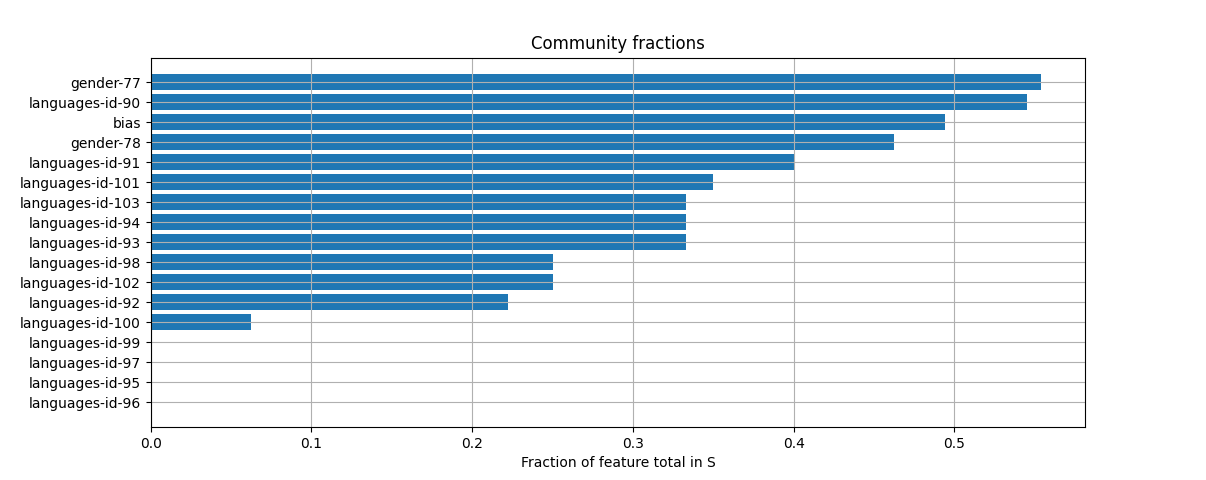
\includegraphics[width=\linewidth]{ego-0-abp-community-fractions.png}
		\caption{Community fractions $|\Omega_i \cap S| / |\Omega_i|$}
		\label{fig:abp-output-community-fractions}
	\end{subfigure}
	\begin{subfigure}{0.6\linewidth}
		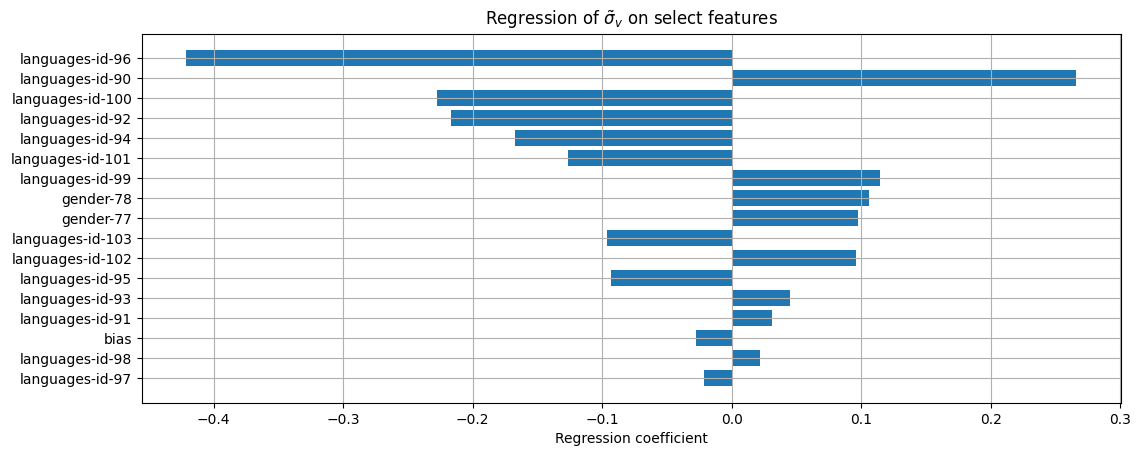
\includegraphics[width=\linewidth]{ego-0-abp-lin-regression.png}
		\caption{Linear regression of $\tilde{\sigma}_v$ on select feature ($R^2 = 0.113$)}
		\label{fig:abp-output-lin-regression}
	\end{subfigure}
	\caption{Egonet-0 linear classifier results}
\end{figure}

\section{Future Direction}

\section{Conclusion}

\nocite{*}
\printbibliography

\end{document}
